\documentclass{article}
\usepackage[utf8]{inputenc}
\usepackage{geometry}
\usepackage{natbib}
\usepackage{pxfonts}
\usepackage{graphicx}
\usepackage{setspace}
\usepackage{hyperref}
\usepackage{lineno}

\doublespacing
\linenumbers

\title{Episodic memory: mental time travel or a quantum `memory wave' function?}
\author{Jeremy R. Manning\\Dartmouth College, Hanover, NH\\jeremy.r.manning@dartmouth.edu}

\begin{document}
\maketitle

\begin{abstract}
Where do we ``go'' when we recollect our past?  When remembering a past event, it is intuitive to imagine some part of ourselves mentally ``jumping back in time'' to when the event occurred. I propose an alternative view, inspired by recent evidence from my lab and others, as well as by re-examining existing models of episodic recall, that suggests that this notion of mentally revisiting any specific moment of our past is at best incomplete and at worst misleading.  Instead, I suggest that we retrieve information from our past by mentally casting ourselves back simultaneously to \textit{many} time points from our past, much like a quantum wave function spreading its probability mass over many possible states.  This revised conceptual model makes important behavioral and neural predictions about how we retrieve information about our past, and has implications for how we study episodic memory experimentally.
\end{abstract}

\section*{Introduction and overview}
How do our brains organize, retrieve, and act upon the ceaseless flow of incoming information and experiences?  \cite{Tulv83} contends that episodic memory is like a sort of ``mental time travel,'' whereby we send some part of our mental state back along our autobiographical timeline to a specific moment in our past.  This view has fundamental implications for how we study and build theories about memory: it suggests that we can match up specific moments of recollection with specific moments from the past.  These implications extend to how we design episodic memory experiments and how we analyze the behavioral and neural data from those experiments in order to understand the neural and/or cognitive mechanisms that underly memory retrieval.  At its core, characterizing episodic memory as mental time travel makes studying and understanding memory about matching.  Specifically, the primary implied questions are about how and when we match up the thoughts (and/or brain activity patterns) we are experiencing at one moment with the thoughts (and/or brain activity patterns) we experienced at another previous moment.  The challenge, then, is to understand the neural (structural) and cognitive (functional) mechanisms that characterize when, how, and why our memory systems allow us to relive those prior experiences.  One way of illustrating how this framing misses out on key aspects of memory is to examine how experimentalists and theorists typically conceive of and model a mental construct called \textit{context}.

The notion of context was fundamental to \citeauthor{Tulv83}'s characterization of episodic recall, and continues to be a primary feature of most current theories of episodic memory~\citep[e.g., for review see][]{Kaha12}.  Whereas the \textit{content} of a memory provides specific information about the episode itself, contextual components of a memory help to frame the episode within the rememberer's broader experience.  Defining context precisely (e.g., as distinct from content) is an ongoing challenge for our field, but theorists generally describe context as reflecting a mental combination of external cues (where you are, who you are with, background sensory information, etc.) and internal cues (thoughts, feelings, emotions, etc.) that uniquely define each moment~\citep[e.g., see review by][]{MannEtal15}.  Reactivating the mental representation of the context associated with a given episode is what can give us the feeling of some ``part of ourselves'' re-experiencing the past.

One practical way to distinguish content from context representations is to separate mental (or neural) representations that drift rapidly \citep[content;][]{PolyEtal05, MannEtal12} or gradually \citep[context;][]{PolyEtal05, MannEtal11, HowaEtal12, LohnEtal18, LongKaha18, FolkEtal18}.  An intuition for why contextual representation might be expected to evolve gradually is laid out by \cite{PolyKaha08}.  Essentially, slowly drifting thoughts may be used to ``index'' more rapidly drifting thoughts that are temporally proximal.  This notion, that our brain maintains parallel mental representations drifting at different time scales, has been well-characterized in a series of elegant fMRI and ECoG studies by Uri Hasson and colleagues~\citep{HassEtal08, LernEtal11, HoneEtal12, AlyEtal18}.  Subsequent work by the same group has shown that this hierarchy of drifting mental representations plays a central role in how we remember continuous experiences and segment our experiences into discrete events~\citep{BaldEtal17}. This work mirrors the discovery of \textit{time cells} in the rodent hippocampus that respond preferentially to a specific time relative to a temporal reference (e.g., time elapsed since starting to run on an exercise wheel), whereby each cell appears to integrate incoming information at a different rate~\citep{PastEtal08, MacDEtal11} and the population activity serves to represent information at a range of timescales~\citep{MauEtal18}. Other work suggests that the lateral entorhinal cortex also plays a role in integrating information across a wide range of timescales~\citep{TsaoEtal18}, supporting precise temporal recall~\citep{MontEtal19}.  These ideas have been formalized in a family of theoretical models over the past several decades~\citep{HowaKaha02, DianEtal07, SedeEtal08, PolyEtal09, ShanEtal09, ShanHowa10, ShanHowa12, HowaEtal14, Rang18}.  In turn, these models were inspired in part by earlier theoretical work suggesting that temporally proximal experiences become linked through their shared contextual features~\citep{Este55a,AtkiShif68}.  Other recent work
indicates that different aspects of the reinstatement process itself might also occur at multiple timescales.  For example, \cite{LindEtal19} found that high-level semantic information was reinstated prior to low-level (e.g. perceptual) details in an associative memory task.  Collectively, these experimental and theoretical studies make two important contributions to our understanding of how we remember our past.  First, the studies suggest that our ongoing experiences are ``blurred out'' in time by neural integrators (where different brain structures or sub-structures integrate with different time constants).  Second, the studies suggest that members of this family of representations drifting at different rates become bound together such that when we retrieve memories about our past, we reactivate representations that carry information at a range of time scales.  These reactivations explain how our brains reactivate prior contexts when we remember the past.

Although reactivating context is often \textit{described} as a sort of mental time travel back to the one specific moment being remembered, there is some apparent inconsistency between this description and how this process is actually characterized mathematically or measured neurally.  In particular, both the theory and neural measures described in the preceding paragraphs characterize episodic recall (mathematically) as reflecting the reactivation of a weighted blend of thoughts from a \textit{range} of previously experienced times-- not to any one \textit{specific} time.  This is not simply a matter of imprecision in mental time travel (i.e., a reflection of the low effective resolution with which we can revisit specific moments from our past).  Rather, when we retrieve the thoughts associated with a range of times, it is conceptually more like we are simultaneously visiting \textit{many} of our prior experiences. The above human and rodent studies suggest that the brain maintains parallel representations of ongoing experience, each drifting at a different timescale.  The notion of thinking of any one particular moment from the past is incompatible with this multiple timescales view, in that our thoughts and brain activity patterns reflect information from a range of moments, even when we are not specifically engaged in remembering.  If what we consider to be a ``moment'' or ``now'' is guided by our neural representations of our ongoing experiences, then this implies we are continually experiencing \textit{many} ``nows.''  If our thoughts are continually spread across a range of times, the notion of mentally revisiting any particular moment loses its meaning.

Where the mental time travel framing breaks down most notably is when we consider scenarios in which the particular blend of timepoints reflected in one's current thoughts do not come from temporally contiguous events.  Understanding how a new experience fits in with our broader understanding might require integrating information gleaned from many experiences separated in time, each with their own contextual attributes.  For example, having an important conversation with a friend might require bringing in information acquired during other interactions with that friend, other conversations about related or similarly important topics, general knowledge about communication styles, etc.  \citep[This notion of bringing a range of prior experiences to bear on guiding our ongoing behaviors is also related to a literature on \textit{situtation models}; for review see][]{RangRitc12}.  That we can integrate information across experiences suggests that the integration of incoming information at different rates need not be a purely mechanical process, but rather may reflect a deeper functional role~\citep[also see][]{BrigEtal18}.  When we simultaneously reactivate thoughts related to separated moments from our past, this provides a means of associating and relating those temporally distinct experiences.  This is how we can integrate information across the \textit{many} discrete experiences relevant to ``now.''

\section*{The temporal dynamics of ongoing experience and how we remember it}
Modern context-based theories of episodic memory posit that the current state of mental context serves to determine which information from our past may be relevant to us and therefore reactivated~\citep[e.g., ][]{PolyEtal09}. Although these theories were largely developed and tested in the domain of list-learning paradigms, conceptually similar principles might also underlie real-world memory.  For example, prior experiences with shared or overlapping contextual properties (e.g., other experiences that occurred in similar spatial or social settings, shared similar goals, etc.) could be leveraged to form schemas or situation models that help guide behaviors and expectations according to the current perceived context~\citep{RangRitc12, BaldEtal18, AlyEtal18}.

Unlike random word lists, naturalistic experiences contain \textit{event boundaries} whereby contextual cues change sharply from one moment to the next, implying a change in the current situation (e.g., shifting from the quiet peace of working on a manuscript in the early morning to the frenzied chaos of helping a newly awoken child get ready for school).  A number of studies (using non-random lists and more naturalistic stimuli) have found that the way we remember past experiences can be shaped by these event boundaries.  For example, controlling for elapsed time, memory is impaired for information that occurred prior to a change in the current event or situation~\citep[e.g., ][]{RadvCope06, SwalEtal09, SwalEtal11, EzzyDava11, MannEtal16}.  The temporal dynamics of contextual change also underlie how we judge the amount of time elapsed since a prior reference point~\citep{BlocReed78, SahaSmit14}.  These findings suggest that the rapid contextual or situational changes that define these event boundaries shape how we experience and remember~\citep{DuBrDava16}, similarly to how spatial boundaries~\citep[e.g., environmental barriers;][]{McKeBuzs16, BrunEtal18} shape how we experience and remember spatial environments and layouts, or how conceptual boundaries~\citep[e.g., distinctions between semantic categories;][]{BrunEtal18} shape how we experience and remember conceptual information.

Event boundaries are one example of the broader temporal covariance structure that is characteristic of ongoing experience.  Whereas classic approaches to studying memory (e.g., list-learning paradigms and other trial-based experiments) encourage researchers to treat each moment, trial, or stimulus as separable from the rest of experience, context-based theories of memory (including situation models and event-based models) posit that each moment derives meaning through its deep ties to other related (but potentially temporally separated) experiences.  This rich tapestry of interacting moments and experiences forms a scaffolding for interpreting our new experiences and for retrieving information concerning our past.  According to this view, the reactivation of this rich tapestry of contextual details enfolding the remembered event (i.e., how the event relates to the rest of one's experiences across timescales) is even more central to our subjective experience than the specific details of what occurred during that event!  This begs the question: which thoughts, from which times, do we reactivate when we remember our past experiences?

\subsection*{How is our past replayed when we remember?}
Our ongoing experiences can cue us to remember information about our past.  This can happen explicitly (e.g., during a conversation about a specific prior event) or implicitly (e.g., when something happening now reminds you of what happened before).  Context-based theories of memory posit that the particular memories that our ongoing experiences cue will be related~\citep[contextually, semantically, functionally, etc.; e.g., ][]{PolyEtal09}.  One potential challenge to studying how we remember the past relates to detangling which links between our experiences are specifically driven by our memory systems versus which are imposed ``externally'' through the similarity structure of those experiences.  For example, consider your daily commute into work.  If you were to verbally recount a specific day's commute later, one might expect some aspects of your description to apply to other days' commutes as well (e.g., other commutes where you took a similar route or travelled via similar modes of transportation, listened to similar music along the way, travelled at a similar time, etc.).  But to what extent could one hope to separate out descriptive matches driven solely by similarities in those commuting experiences, versus true reactivations (in memory) of specific memories of those other prior commutes?

One insight into this distinction comes from a recent study by \cite{HeusEtal18c}, which analyzed data collected by \cite{ChenEtal17} who had participants watch an episode of the BBC television show \textit{Sherlock} and then verbally recount what happened in the episode.  The authors used topic models~\citep{BleiEtal03} applied to human-generated annotations of each camera shot in the episode to characterize the episode's content with a timeseries of high-dimensional semantic feature vectors.  These \textit{topic vectors} describe the mix of ``themes'' present in each moment of the episode.  When characterized in this way, the episode's content exhibits periods of relative stability, followed by moments of rapid change. This interplay between stability and change is visible as ``blocks'' in the temporal correlation matrix (Fig.~\ref{fig:corrmats}A); \cite{HeusEtal18c} performed detailed analyses of these putative \textit{events} and how they are remembered.  Notably, the off-diagonal entries of the temporal correlation matrix (which reflect content similarity between temporally distant events in the episode) are nearly all close to 0.  This is surprising, because the episode itself comprises a murder mystery with recurring motifs that must be associated in the viewer's mind in order to make sense of the episode.  Nonetheless, when considering solely the semantic content of each moment of the episode, those long timescale associations are nearly entirely absent.  To the extent that this finding extends to real-world experiences, it comports with Heraclitus' notion that one cannot step in the same river twice~\citep{Hera}.

\begin{figure}[tp] \centering 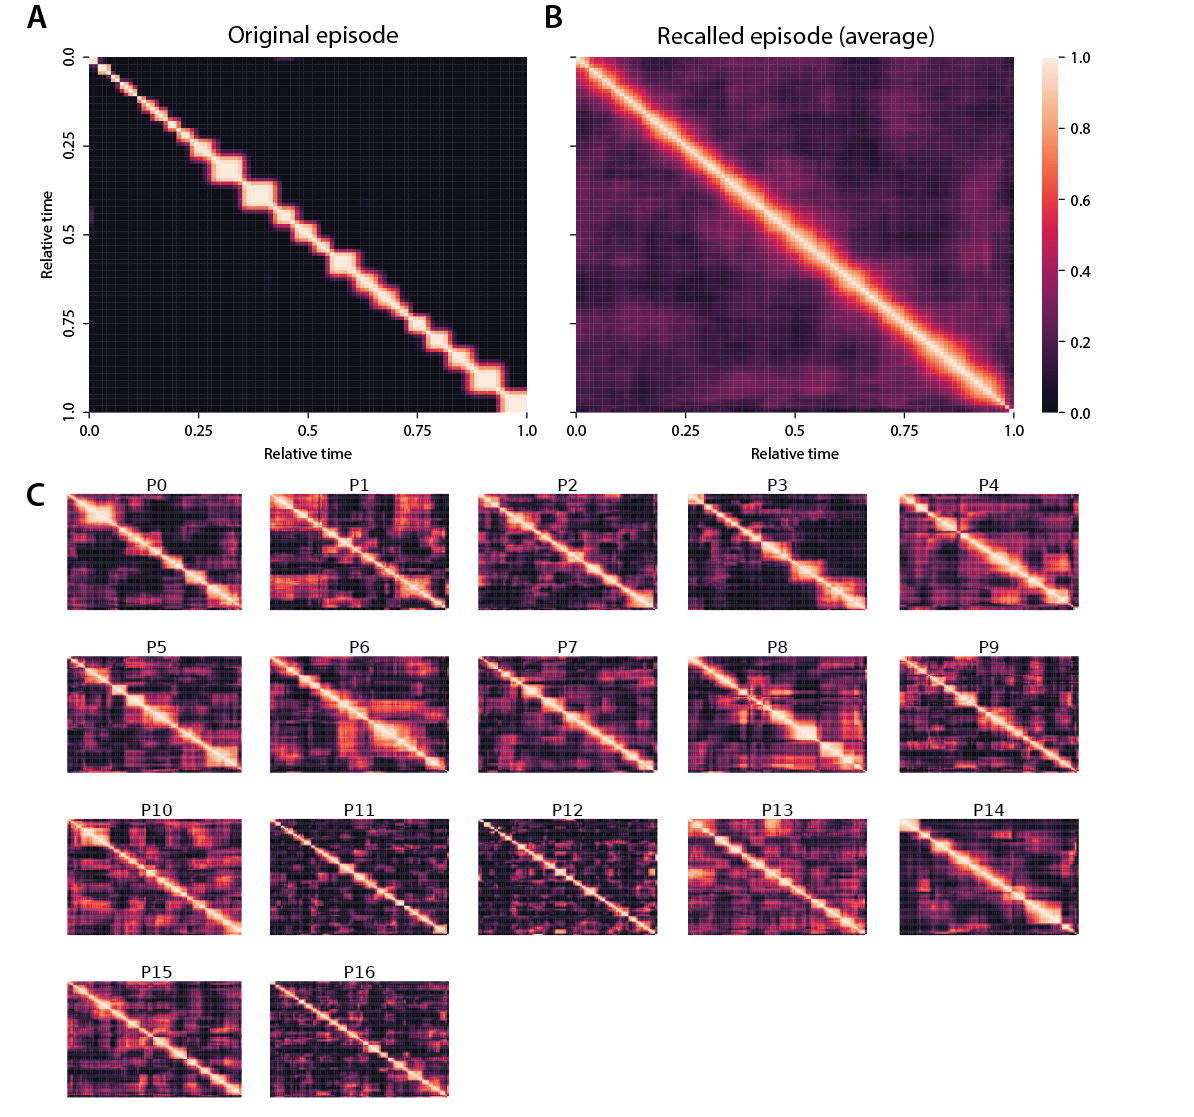
\includegraphics[width=0.8\textwidth]{figs/pres_rec_corrmats_sherlock.png} \caption{\textbf{Temporal correlation matrices of the dynamic content of a television episode and people's recalls of that episode.}  The panels of this figure are adapted from \cite{HeusEtal18c}, where full details may be found. \textbf{A. Temporal correlations exhibited by the content of the television episode.}  Each moment of an episode of the BBC television show \textit{Sherlock} has been characterized using a topic model~\citep{BleiEtal03} fit to detailed human-generated annotations between each scene cut.  The correlations between the topic vectors of a given pair of timepoints reflects the similarity in thematic content at those timepoints.  \textbf{B. Temporal correlations exhibited by the (average) content of participants' recalls of the episode.} The topic model used to characterize the episode in Panel A has been applied to each sentence from each participants' recall transcript.  The temporal correlation matrices describing each participants' recalls were re-sampled using cubic interpolation to have 100 rows and columns prior to averaging the resampled matrices across participants.  \textbf{C. Temporal correlations in the content of individual participants' recalls of the episode.} Each sub-panel displays the temporal correlation matrix for one experimental participant.}
\label{fig:corrmats}
\end{figure}

Although the specific mix of contents in each moment of the episode is nearly unique, participants' subjective experiences of the episode entail weaving together those temporally separated moments into a cohesive narrative.  This is reflected in how people verbally recount the episode later.  If we examine the temporal autocorrelation matrices of participants' recalls of the television episode (characterized using the same topic model used to capture the content of the episode; Figs.~\ref{fig:corrmats}B, C), we see a different structure than that of the episode itself.  Although individual participants' recalls exhibit periods of content stability punctuated by rapid change (block diagonal structure of the matrices in Fig.~\ref{fig:corrmats}C), the off-diagonal correlations between the thematic content of temporally distant events are substantially stronger in participants' recalls than in the original episode.  Another way of characterizing this phenomenon is to look at the autocorrelation functions (describing the correlation between different moments' topic vectors as a function of their temporal distance) for the episode and participants' recalls (Fig.~\ref{fig:reinstatement}A).  Whereas the autocorrelations in the original episode's content rapidly fall to 0, autocorrelations in the content of participants' recalls appear to asymptote around an average of 0.2.  These analyses indicate that the way participants \textit{recount} temporally separated events imposes additional similarity on those events, beyond what was present in the original events themselves.  One can then ask: is this simply a matter of imprecision in recall, either with respect to participants' recalls themselves, or with respect to the quality with which they are characterized via semantic feature vectors?  Or might there be a functional role of that additional imposed similarity structure?

To understand which specific events are described (during recall) as more similar than what their original experiences (as characterized by their topic vectors) would suggest, it can be helpful to examine individual recalls of particular events throughout the episode.  Figure~\ref{fig:reinstatement}B displays, for a representative example recalled moment, which other moments from the episode were characterized in a similar way by the participants when they recounted the episode later (black and colored lines), and which other moments in the episode were described in a similar way in moment-by-moment (non-recall) human annotations (gray line).  The example event explored in the figure comprises a scene where Sherlock Holmes and John Watson (main characters) are bantering, and then are interrupted when Sherlock realizes that another victim has been murdered.  The language used by human annotators describing the moment-by-moment contents of the scene used a similar mix of themes only for moments in the episode that were temporally proximal to the event in question (gray line).  However, the way participants described what happened when they \textit{recounted} the episode later revealed a much different pattern.  Specifically, their language mirrored that used when they were recalling other murders, and other moments when Sherlock and John were bantering with or about each other (Fig.~\ref{fig:reinstatement}C).  The way they described the example event did \textit{not} mirror the way they described other semantically (but not conceptually) related events, such as events involving unrelated violence, or Sherlock and John interacting with other characters about other subjects.  Taken together, this suggests that these specific events were associated in participants' memories, perhaps contributing to (or reflecting) their understanding that those events were linked in the episode's narrative.

\begin{figure}[tp] \centering 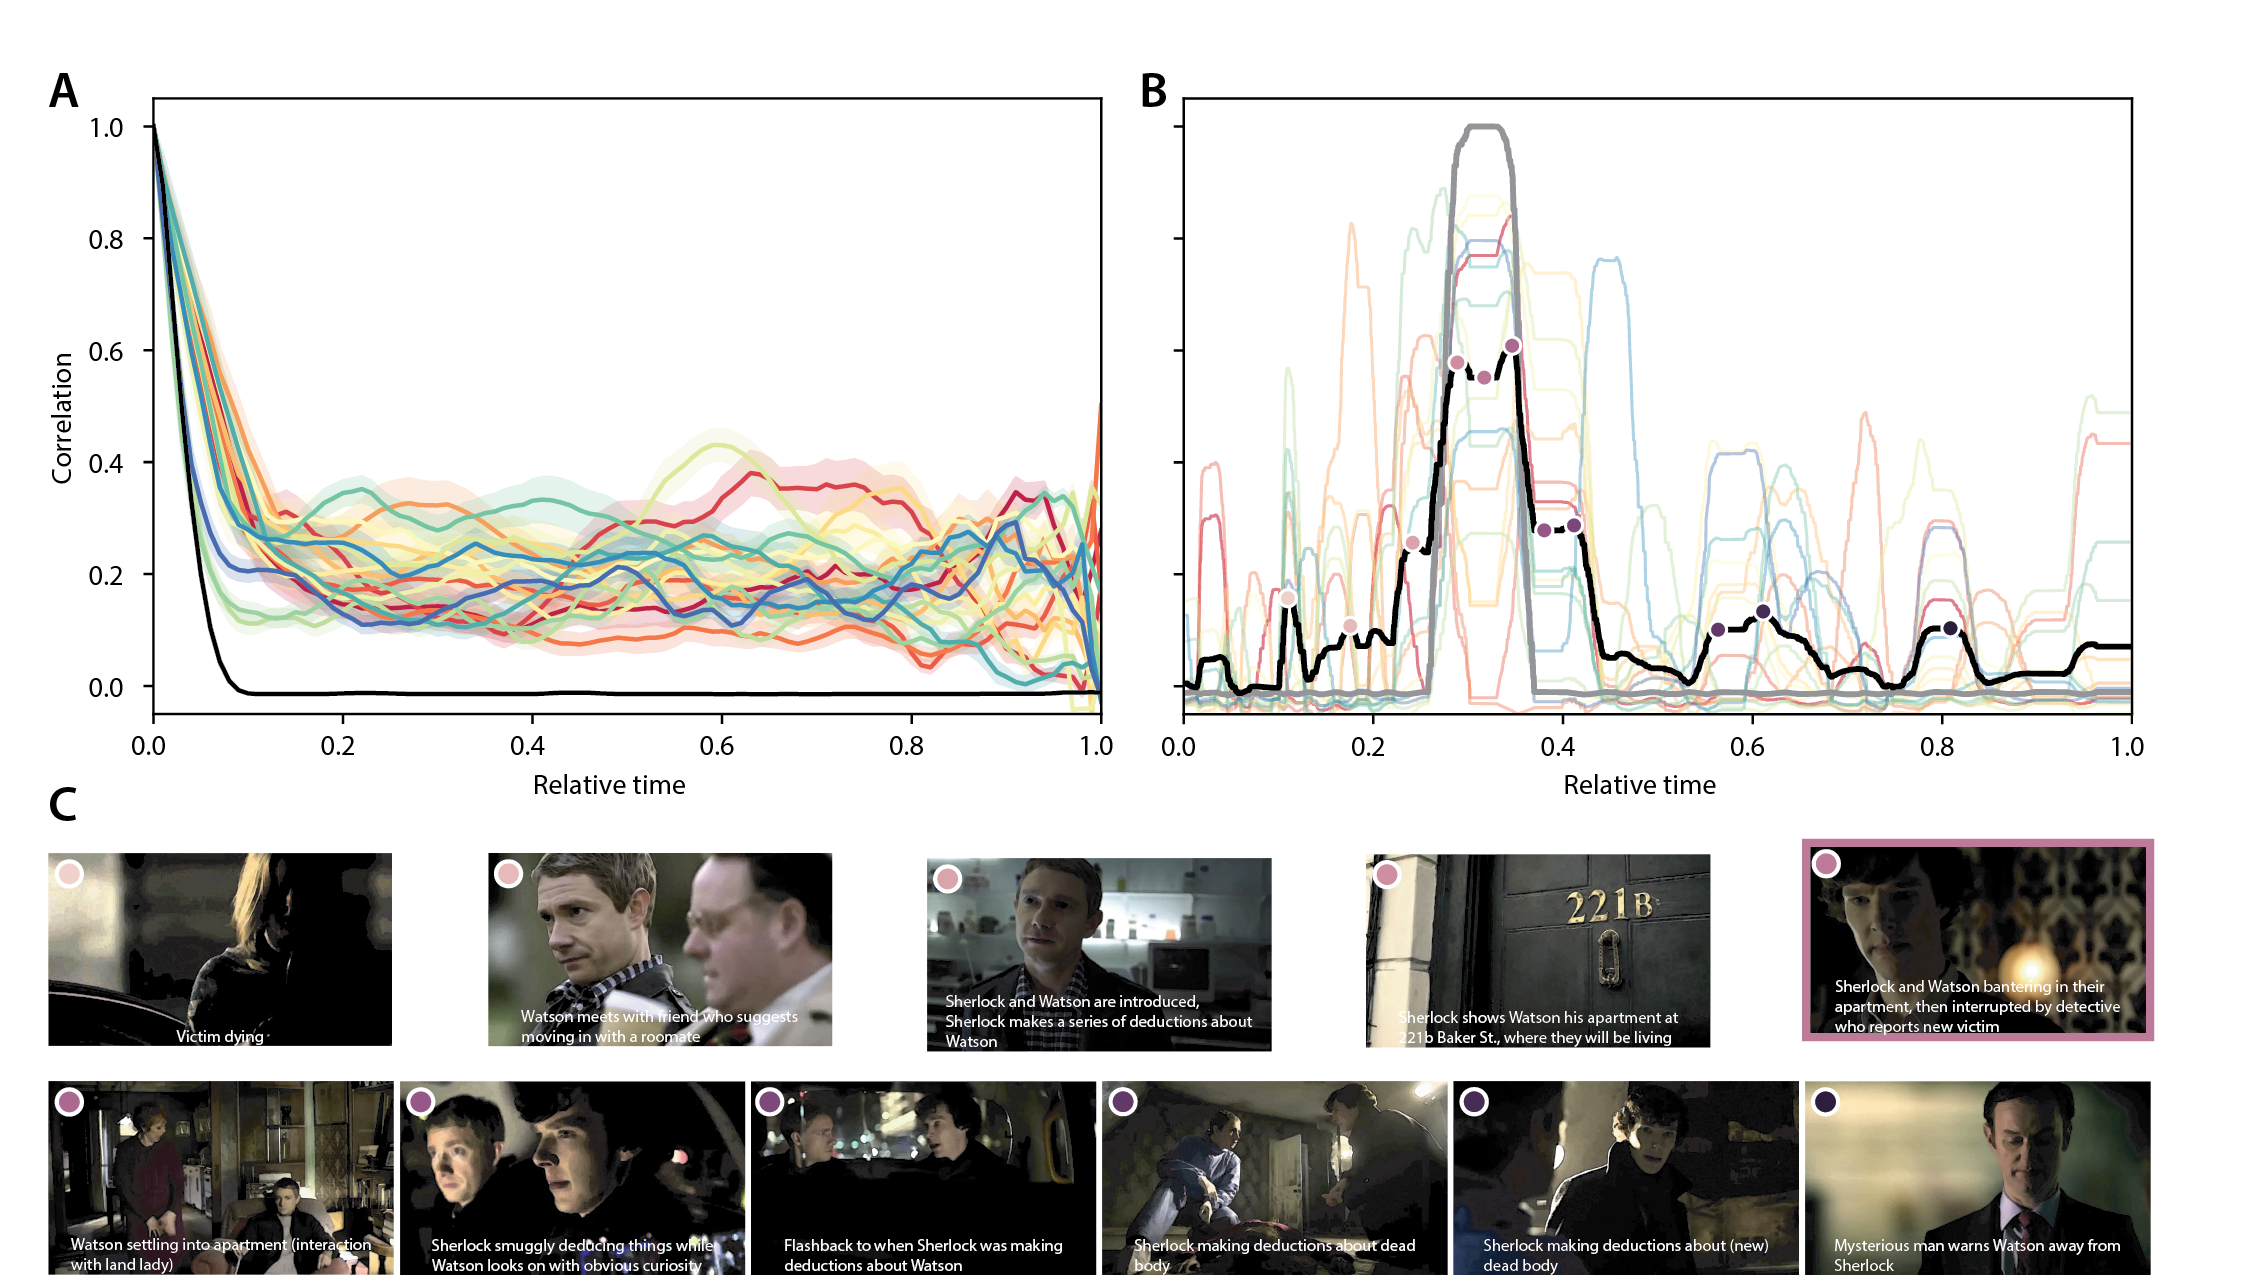
\includegraphics[width=\textwidth]{figs/reinstatement.png} \caption{\textbf{Content drift in a television episode and participants' recalls of that episode.  A.  Autocorrelations in the episode's content and in the content of participants' recalls.}  The black line denotes the average correlations between the topic vectors from pairs of moments in the episode as a function of their temporal separation (times are relative to the full length of the episode).  Each colored line denotes an analogous autocorrelation function, but for each individual participant's recalls of the episode (times are relative to the full length of each participant's recalls).  The error ribbons denote 95\% confidence intervals, taken across all moments in the episode (or in participants' recalls of the episode).  \textbf{B. Recall density functions for one recalled moment.} Each curve reflects the correlations between the topic vector at each (relative) moment of the episode (or participants' recalls of the episode), and the topic vector of an event beginning approximately $\frac{1}{3}$ through the episode (relative time: 0.328).  The gray curve denotes these correlations for the topic vectors derived from annotations of the episode itself. The black line denotes the average correlations across all participants' recalls.  Local maxima are marked with colored dots.  Local maxima closer than 2.5\% of the total recall duration to a higher local maximum were excluded (this constraint served to eliminate very nearby peaks that corresponded to duplicate events), as were maxima with peaks with correlation coefficients lower than 0.1 (this threshold was chosen arbitrarily; this constraint served to eliminate events that were only very weakly associated with the example event).   The colored lines denote the correlations for each individual participant's recalls.  \textbf{C. Local maxima in the average recall density function.}  Representative screen captures from the scenes at each local maxima in Panel B are displayed (dot colors match those in Panel B).  The text in each screen capture displays a brief summary of what happened in each scene. The colored outline denotes the reference scene being recalled.}
  % colors: individual participants
  % black: average across participants
  % gray: autocorrelation with topic vector at timepoint
  % circles: local maxima in the across-participants average (i.e., movie events that share structure with the given timepoint that is distinct from other temporally proximal events)
\label{fig:reinstatement}
\end{figure}

A rich recall density function analogous to the one displayed in Figure~\ref{fig:reinstatement}B could, in principle, be characteristic of memory for \textit{any} past event or experience.  For example, the peaks of the function could provide insight into which events, from which moments along one's autobiographical timeline, are functionally associated in memory.  Nonetheless, a potential challenge to testing this hypothesis in the laboratory is that in many memory studies there is no particular reason for participants to functionally associate the stimuli.  For example, there is often no ``deeper narrative'' to make sense of in list-learning studies or in most standard trial-based memory experiments.  However, random word list learning experiments might happen to contain (for a given list) semantically related words.  Indeed, a number of studies indicate that participants spontaneously form associations between semantically related words on random word lists, even when those related words are separated in time~\citep[e.g.,][]{WixtRohr94, MannKaha12, MannEtal12}.  This suggests that our memory systems pick up on statistical regularities, even in ostensibly ``random'' stimulus sequences, and that we leverage those regularities when we recall our past~\citep{PolyEtal09}.  Other work suggests that our memory systems may also leverage these regularities to parse our ongoing experiences into discrete events~\citep{SchaEtal13, Shap19}.  Are these examples in the literature on random list learning studies, indicating that our memory systems leverage ``accidental'' structure in random sequences, a reflection of the same fundamental principle driving the sorts of memory reactivation function displayed in Figure~\ref{fig:reinstatement}B?

It is difficult to explicitly test whether (apparent) semantic reinstatement in word list learning, as reflected in people's tendencies to semantically cluster recalls of random word lists, reflects integration of information across the experiences of studying those words.  However, remembering word lists does not \textit{require} integrating information across words in order to specifically gain a deep understanding of the list.  By design, there \textit{is} no deeper meaning of random word lists.  One way to characterize the meaning reflected by how an experience unfolds in time is through models that describe the geometric path that the experience takes through an appropriate representational space.


\section*{The shapes of remembered experiences}
The study by \cite{HeusEtal18c} described above suggests one way of characterizing the dynamic content of complex naturalistic stimuli like television episodes.  The sequence of topic vectors over the course of the episode traces out a \textit{topic trajectory} through a high-dimensional feature space.  The sequence of topic vectors for a given participant's recalls traces out an analogous trajectory.  This characterization provides a geometric framework for comparing the \textit{shapes} that reflect how naturalistic experiences unfold over time, to the shapes of how we remember those experiences later (Fig.~\ref{fig:trajectories}).  One can then use the geometric transformations needed to map an experience's trajectory onto the trajectory of its later remembering to characterize the quality and content of memory.

\begin{figure}[tp]
\centering
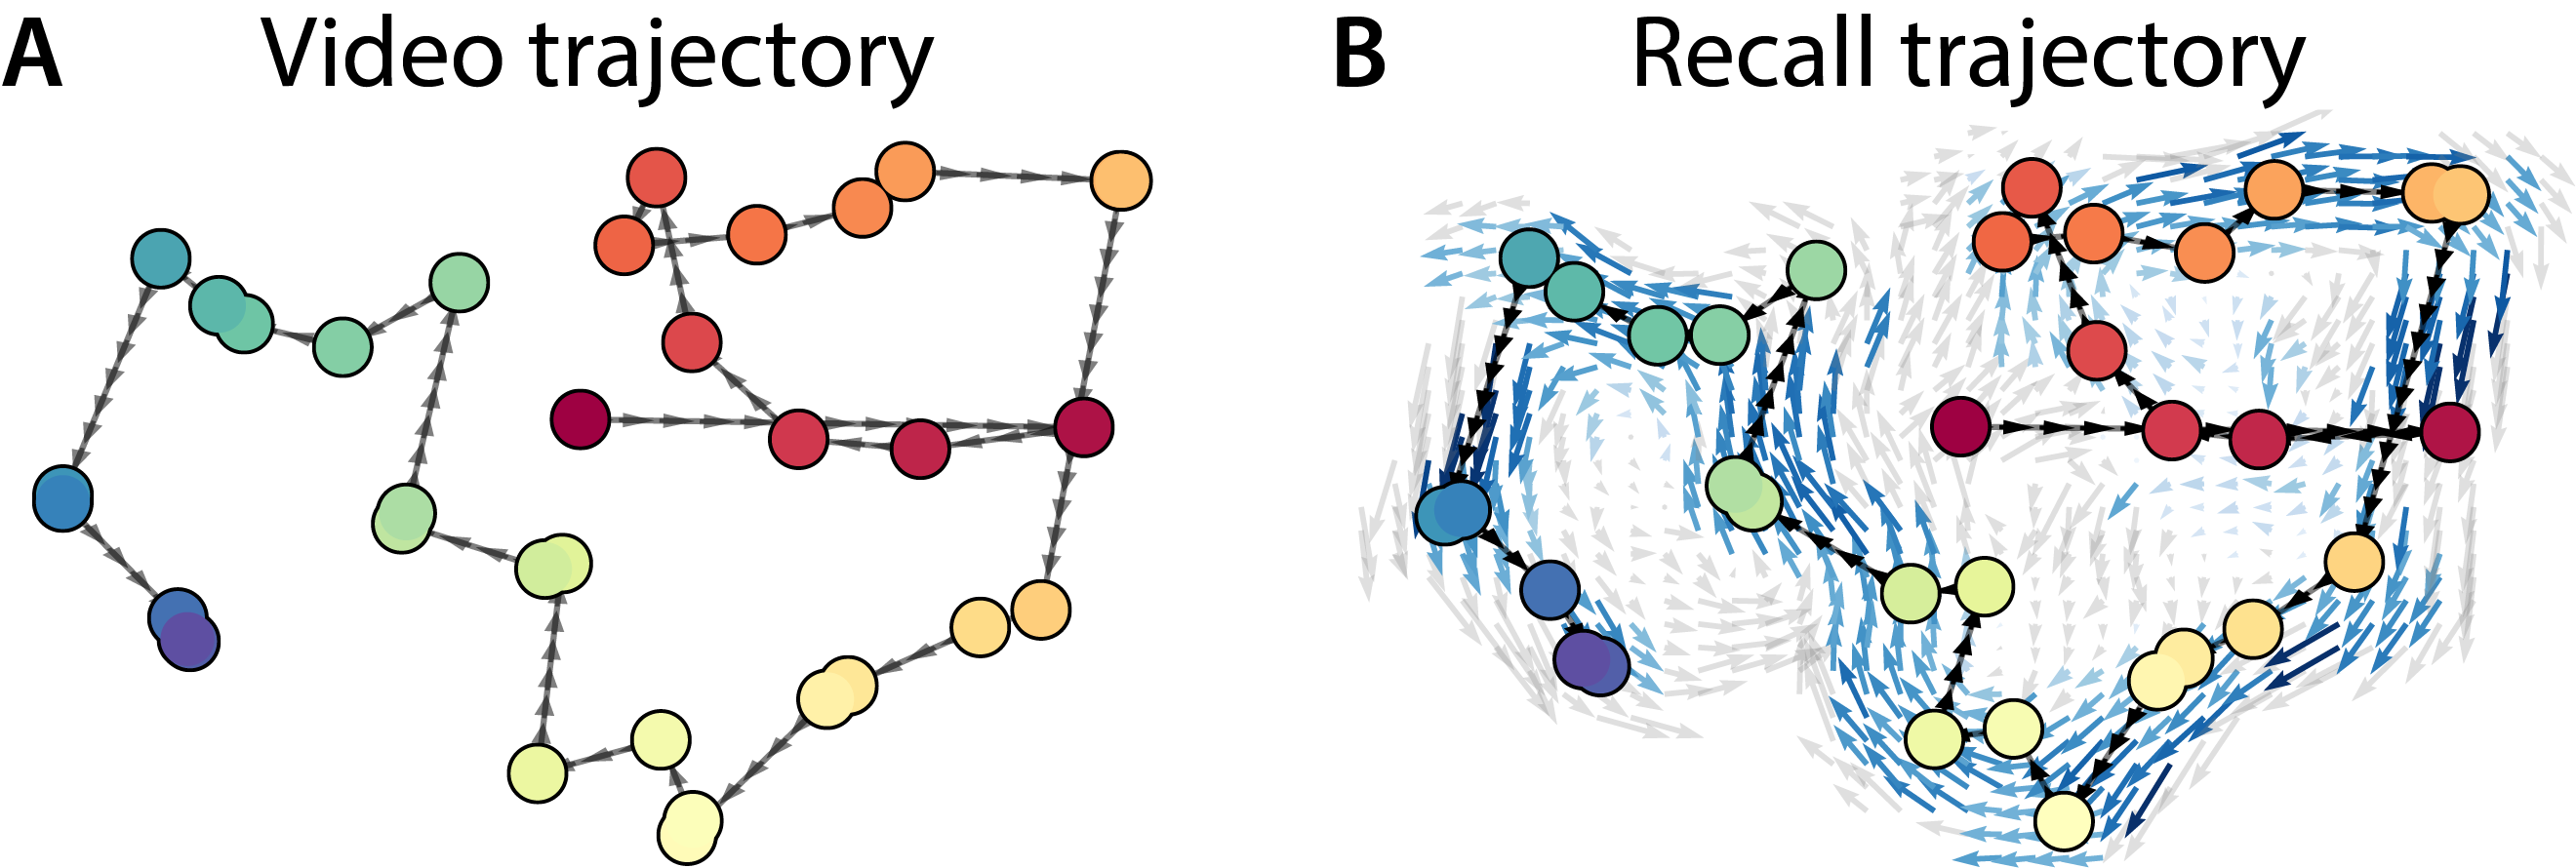
\includegraphics[width=0.8\textwidth]{figs/trajectory.png}
\caption{\textbf{The shape of an unfolding experience.}  \textbf{A. The trajectory through topic space taken by a television episode.} The topic trajectory taken by a 50 minute television episode, projected onto two dimensions.  Each dot indicates an event identified using a Hidden Markov Model; the dot colors denote the order of the events (early events are in red; later events are in blue), and the connecting lines indicate the transitions between successive events.  \textbf{B. The trajectory through topic space taken by participants' recalls of the television episode.} The average two-dimensional trajectory captured by 17 participants' recalls of the episode, with the same format and coloring as the trajectory in Panel A. The arrows reflect the directions of the average transitions taken by participants whose trajectories crossed that part of topic space; blue denotes reliable agreement across participants.  Figure adapted from \cite{HeusEtal18c}, where additional details may be found.}
\label{fig:trajectories}
\end{figure}

In addition to serving as a framework for quantifying the dynamic content of experiences, these trajectories may be visualized geometrically by projecting word embedding representations of the events onto lower dimensional spaces~\citep[e.g., ][]{HeusEtal18a}; for additional discussion and counterpoints see~\cite{JollChan18}.  \cite{HeusEtal18c} applied this approach to the same dataset reflected in Figure~\ref{fig:trajectories}, revealing another key property of how we remember.  Although there are substantial individual differences in the specific words people use to describe their shared experience of watching the same television episode, and how much detail they recollected, the overall shapes of those recalled experience trajectories are highly similar across people.  This has potentially exciting implications for what it means to communicate memories to other people: we need to convey the ``gist'' (shape) of our experience.  It also has implications for how we learn by analogy: perhaps events that share schemas~\citep[e.g., ][]{BaldEtal18}  unfold in similar ways (e.g., have similar shapes).  Learning which shapes go with which schemas could provide a scaffolding for rapid learning and generalization of new experiences, to the extent that those new experiences match a previously learned schema (shape).


\subsection*{Extensions to spatial, semantic, affective, and social representations}
Just as we mentally spread ourselves across a distribution of times when we remember, we can perform similar mental operations when we conceptualize and retrieve other types of information.  Further, these distributions may be estimated using existing methods.  For example, consider how we use pattern classifiers~\citep{NormEtal06b} to connect neural activity patterns to specific semantic~\citep{PolyEtal05, MitcEtal08, MannEtal12}, spatial~\citep{MillEtal13}, affective~\citep{ChanEtal18}, and social~\citep{MeyeEtal18} content being mentally manipulated.
A prevailing approach is to label specific brain activity patterns as each reflecting \textit{one particular} concept or mental state.  Variability in neural activity over repeated experiences or rememberings can result in classifiers spreading their predictions over multiple possible mental states.  Traditional approaches then ``clean up'' this distribution over possible mental states by taking its average (expected), maximum, or modal value.  However, following the ``quantum wave function'' logic described in this manuscript, I suggest that the specific shape of these distributions may not only be informative, but they are \textit{more accurate reflections of what our neural activity patterns actually reflect}.  What are some implications of this view for non-memory domains?

One example of how the full distribution over possible mental states can provide insights into cognition may be seen in how the brain encodes spatial locations.  Theoretical~\citep[e.g., ][]{GersAbbo97} and empirical~\citep[e.g., ][]{PfeiFost13} work has demonstrated how place cell receptive fields may be modulated according to environmental features such as obstacles and the locations of rewarded goals.  In other words, although place cells encode an animal's location within an environment, even for a fixed cell and environment there is some variability with respect to where precisely within that environment the cell modulates its firing rate.  These studies suggest that variability in the set of locations to which a place cell responds is not merely a reflection of noise or imprecision.  Rather, this variability might have some functional relevance in terms of facilitating the learning of paths around obstacles and towards goals.

The notion that variability and ``uncertainty'' can be informative also has implications for how our brains might efficiently represent information.  Recent work suggests that adversarial networks trained to learn a generative model of natural images~\citep[e.g., ][]{GatyEtal16, IsolEtal17} may be used to refine estimates of decoded visual stimuli~\citep{StYvNase18}. Related manifold learning approaches that ``snap'' decoded estimates to the nearest surface location on a learned manifold may be used in a similar way to decode sequences of movie frames~\citep{HeusEtal18a}.  Taken together, these findings suggest that not all \textit{possible} images (and by extension, all possible stimuli) are equally likely.  Rather, the set of stimuli likely to be encountered live within subspaces or on manifolds in the relevant representational space.  The geometry of these manifolds provides insights into the statistical structure of the stimuli.  It also provides potential insights into how the brain represents those stimuli, for example to the extent that the geometries of these manifolds may be leveraged to improve brain decoding.  The shapes of these manifolds can potentially provide insights into how our thoughts are distributed over representational spaces.

\section*{Concluding remarks}
When we remember an experience, we bring back thoughts related to a range of other semantically, conceptually, and functionally related experiences.  This can serve an important functional role: it allows us to integrate information across temporally separated experiences.  Although this view is captured mathematically by context-based theories of episodic memory, it is \textit{not} specifically captured by the conceptual notion of mental time travel that is often used to describe episodic recall.  The alternative conceptualization presented here, that when we remember our past we reinstate thoughts associated with a weighted blend of our prior experiences, also has links with non-temporal or episodic domains such as semantic, spatial, affective, and social representations.  Characterizing how our thoughts reflect \textit{distributions} over representational spaces is central to understanding how we think about ourselves, our experiences, other people, and the world around us.

\section*{Acknowledgements}
I thank Luke Chang, Janice Chen, Paxton Fitzpatrick, Andrew Heusser, Christopher Honey, Talia Manning, Lucy Owen, Matthijs van der Meer, and Kirsten Ziman for feedback and scientific discussions. I also thank Janice Chen, Yuan Chang Leong, Kenneth Norman, and Uri Hasson for sharing the data re-analyzed here, and Paxton Fitzpatrick and Andrew Heusser for contributing analysis code that I adapted from a prior publication.  This work was supported in part by NSF EPSCoR Award Number 1632738. The content is solely my responsibility and does not necessarily represent the official views of my supporting organizations.

\section*{Data and code availability}
All analysis code and data used in the present manuscript may be found \href{https://github.com/ContextLab/mental-time-travel-paper}{\underline{here}}.

\bibliographystyle{apa}
\bibliography{CDL-bibliography/memlab}
\end{document}
